\chapter{Dise\~no metodol\'ogico}
\label{sec:diseno}
\section{Hip\'otesis}
?`Es posible desarrollar una herramienta inform\'atica que automatice la 
tarea de encontrar una lista de procesos judiciales en diferentes documentos
de notificaciones por estado de distintos juzgados?.
\section{Tipo de investigaci\'on}
Esta investigaci\'on tomar\'a un enfoque cuantitativo.
\section{Poblaci\'on}
Los documentos impresos de notificaciones por estado de los juzgados civiles municipales de menor cuant\'ia de la ciudad de Pereira.
\section{Unidad de an\'alisis}
Fotograf\'ias de los documentos mencionados en la poblaci\'on.
\section{Muestra}
La muestra est\'a compuesta por las fotograf\'ias de estados y traslados de los juzgados civiles municipales de Pereira de los d\'ias:
\begin{itemize}
\item 19 de septiembre de 2013.
\item 20 de septiembre de 2013.
\item 24 de septiembre de 2013.
\item 25 de septiembre de 2013.
\item 26 de septiembre de 2013.
\item 27 de septiembre de 2013.
\item 07 de octubre de 2013.
\item 08 de octubre de 2013.
\item 09 de octubre de 2013.
\item 11 de octubre de 2013.
\item 15 de octubre de 2013.
\item 21 de octubre de 2013.
\item 22 de octubre de 2013.
\item 23 de octubre de 2013.
\item 24 de octubre de 2013.
\item 25 de octubre de 2013.
\item 28 de octubre de 2013.
\item 29 de octubre de 2013.
\item 30 de octubre de 2013.
\item 31 de octubre de 2013.
\item 01 de noviembre de 2013.

\end{itemize}
\section{Variables}
Las variables ser\'an las siguientes:
\begin{itemize}
\item Porcentaje de coincidencias reconocidas correctamente en total.
\item Porcentaje de coincidencias reconocidas por cada juzgado.
\item Porcentaje de seguridad con el que se reconoci\'o cada proceso.

\end{itemize}
\section{Dise\~no de instrumentos}
Para determinar el porcentaje de coincidencias reconocidas por juzgado 
se usar\'a el formato especificado en la figura \ref{fig:coincidencias_por_juzgado}, 
donde se pueden registrar f\'acilmente la cantidad de procesos que se 
notifican por estado diariamente, los procesos que debe reconocer y las
coincidencias reconocidas, para que de esta manera se pueda registrar un
porcentaje de reconocimiento diario y total correspondiente a todos los 
d\'ias medidos para ese juzgado. 

\begin{figure}[h]
\begin{center}
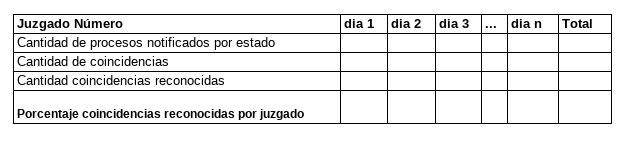
\includegraphics[scale=0.7]{./porcentaje_coincidencias_por_juzgado.png}
\end{center}
{\caption{Instrumento para determinar el porcentaje de coincidencias reconocidas por juzgado.}\label{fig:coincidencias_por_juzgado}}
\end{figure}

\paragraph{}
Para determinar el total de coincidencias reconocidas se usar\'a el 
formato descrito en la figura \ref{fig:coincidencias}, donde se pueden identificar f\'acilmente 
el total de coincidencias resultantes de la medici\'on en cada juzgado y
el total de coincidencias reconocidas para que de esta forma se pueda 
identificar el porcentaje total.
\paragraph{}

\begin{figure}[h]
\begin{center}
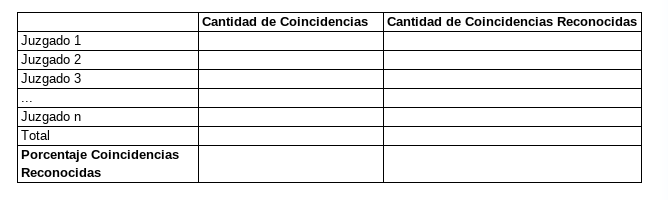
\includegraphics[scale=0.7]{./porcentaje_coincidencias.png}
\end{center}
{\caption{Instrumento para determinar el total de coincidencias reconocidas.}\label{fig:coincidencias}}
\end{figure}

Para medir el porcentaje de reconocimiento acertado por proceso, se 
usar\'a el formato descrito en la figura \ref{fig:coincidencias_por_proceso}, el cual permite registrar 
claramente el proceso donde se ha reconocido una coincidencia, el d\'ia y
el porcentaje de reconocimiento que se identific\'o para este caso.

\begin{figure}[h]
\begin{center}
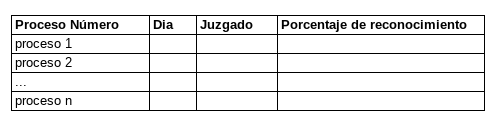
\includegraphics[scale=0.7]{./porcentaje_coincidencias_por_proceso.png}
\end{center}
{\caption{Instrumento para determinar el porcentaje de reconocimiento acertado por proceso.}\label{fig:coincidencias_por_proceso}}
\end{figure}

\clearpage
\pagebreak